\RequirePackage[T1]{fontenc}
\documentclass[conference]{IEEEtran}
\usepackage{cite}
\usepackage{amsmath,amssymb}
\usepackage{graphicx}
\usepackage{url}
\newcommand{\ObservationCount}{3780}
\newcommand{\ConfigurationCount}{252}
\newcommand{\SeqLarge}{37.318}
\newcommand{\OmpLarge}{5.996}
\newcommand{\CudaLarge}{9.839}
\newcommand{\TileLarge}{9.542}
\newcommand{\ModelError}{6.13}
\newcommand{\CannySeq}{1083.075}
\newcommand{\CannySixteen}{203.268}
\newcommand{\HtoDLarge}{1.334}
\newcommand{\KernelLarge}{0.531}
\newcommand{\DtoHLarge}{2.746}
\newcommand{\TileKernelLarge}{0.767}
\newcommand{\HybridHalf}{6.528}
\newcommand{\HybridGpu}{9.119}
\newcommand{\HybridCpu}{6.819}
\newcommand{\RegretMax}{89.35}
\newcommand{\OverlapCount}{5}
\newcommand{\OverlapMax}{0.0556}
\title{A Performance Characterization of CPU--GPU Edge Detection using OpenMP and CUDA}
\author{\IEEEauthorblockN{Author information pending}
\IEEEauthorblockA{Affiliation and contact information pending\\Research draft: human review required before submission}}
\begin{document}
\maketitle
\begin{abstract}
Accelerating an edge-detection kernel does not necessarily reduce host-visible image-processing latency. We characterize sequential C++, OpenMP, CUDA, shared-memory Sobel, and row-partitioned CPU--GPU Sobel on an Intel Core i7-13700HX and NVIDIA RTX 4060 Laptop GPU. A custom Canny variant provides a contrasting CPU workload with global hysteresis. Three procedural grayscale families at four resolutions yield \ObservationCount{} retained observations across \ConfigurationCount{} configurations, with output validation outside every timed interval. At $4096\times4096$, pooled median Sobel latency is \SeqLarge{} ms sequentially, \OmpLarge{} ms with eight OpenMP threads, and \CudaLarge{} ms for baseline CUDA including staging and transfers. Shared-memory tiling increases measured kernel time in the tested configurations. Hybrid results depend on resolution and measurement context; a simple fitted partition model has \ModelError{}\% mean absolute percentage error on the held-out largest resolution. These are bounded, single-session characterization results, not a novel scheduler or a claim of general GPU superiority. The accompanying artifact preserves individual timings, source hashes, analysis scripts, and explicit algorithm and timing contracts.
\end{abstract}
\begin{IEEEkeywords}
edge detection, Sobel, Canny, OpenMP, CUDA, heterogeneous computing, performance characterization
\end{IEEEkeywords}

\section{Introduction}
Edge detection offers a useful contrast between regular local computation and multi-stage processing with global connectivity. A Sobel output depends on a small neighborhood, making spatial partitioning straightforward. Canny adds smoothing, nonmaximum suppression and hysteresis, so distributing individual stages or image regions introduces different correctness obligations. Canny's original formulation emphasizes detection and localization rather than a particular parallel implementation~\cite{canny1986}.

For a discrete GPU, a short convolution can finish quickly while host staging, transfers and synchronization dominate application-visible latency. The CUDA programming model exposes parallelism and memory hierarchy~\cite{nickolls}; it does not guarantee that offloading every image is profitable. Multicore CPU execution is an essential comparison, rather than relying only on a sequential baseline. Benchmark diversity and communication accounting are central concerns in heterogeneous evaluation~\cite{rodinia}.

We ask how image size, CPU thread count, CUDA launch configuration and CPU row fraction affect latency under an identical Sobel contract. The study contributes a reproducible implementation and measurement artifact, an explicit comparison of kernel and pipeline timing, and a held-out diagnostic model of candidate row allocations. It does not claim a new edge detector, a new CPU--GPU partitioning principle, or an exhaustive optimization search. Prior work already addresses adaptive mapping and cooperative image processing. Our scope is a controlled course-project characterization on one commodity laptop.

\section{Related Work}
Luo and Duraiswami implement complete CUDA Canny, including hysteresis, and compare against CPU software~\cite{luo2008}. Emrani et al. evaluate several detectors and replace a breadth-first procedure with a parallel approach~\cite{emrani2017}. Mochurad studies CUDA Canny with image-size and noise-related analysis~\cite{mochurad2022}. Song et al. compare serial, OpenMP, CUDA and OpenCL Canny and investigate access and launch organization~\cite{song2024}. These works preclude a novelty claim based simply on GPU edge detection or comparing programming models. Canny variants also differ in smoothing, thresholding and connectivity; published speedups are not directly transferable to our implementation.

Chang et al. optimize a four-direction $5\times5$ Sobel operator using warp primitives and prefetching on two GPU platforms~\cite{chang2023}. That operator differs from our two-direction $3\times3$ L1-magnitude workload. Stencil auto-tuning~\cite{datta} and Halide's separation of image algorithms from schedules~\cite{halide} establish that locality transformations and execution schedules are longstanding optimization topics. Shared memory is therefore an experimentally evaluated candidate here, not an asserted contribution.

Qilin uses adaptive CPU--GPU mapping~\cite{qilin}. StarPU supplies heterogeneous task scheduling and data management~\cite{starpu}; SKMD partitions OpenCL kernels while accounting for transfers and device performance~\cite{skmd}. Cooperative CUDA execution~\cite{hybrid2014}, Fluidic Kernels~\cite{fluidic}, and performance-aware image-analysis scheduling~\cite{teodoro} further establish this field. A survey organizes cooperative CPU--GPU techniques~\cite{survey2018}. Particularly close recent work by Huang et al. models stage-level CPU/GPU Canny configurations with explicit transfer costs and latency objectives~\cite{recent2026}. Our small row-split model is substantially narrower and is not a replacement for these systems.

Roofline relates performance to computation and data movement~\cite{roofline}, but our measurements do not include the counters required for a quantitative roofline diagnosis. Performance-evaluation work warns about setup bias~\cite{measurementbias} and the need to characterize variability~\cite{georges}. We therefore preserve all observations and report descriptive summaries without statistical-significance claims. The artifact contains a 21-publication review matrix, with full-text and abstract-only evidence distinguished.

\section{Problem Formulation and Research Questions}
Let an image contain $N=WH$ grayscale samples and let $f\in[0,1]$ denote the fraction of rows assigned to the CPU. Our principal metric is steady-workspace wall latency: host input and output exist, reusable device and pinned buffers have been allocated, and processing includes staging, transfers, computation, synchronization and output merging. File I/O, image generation, context creation, allocation of the reusable workspace, and correctness comparison are excluded. This is not cold-start application latency.

We investigate three questions. RQ1: how does OpenMP scaling differ between local Sobel and multi-stage Canny? RQ2: do shared-memory Sobel kernels improve kernel time or host-visible latency? RQ3: when do row partitions improve over device-only execution, and how well can a small model extrapolate to a larger image? The hypotheses are that overhead matters most for small inputs, that tiling need not help a small stencil, and that an allocation based on full-image rates need not minimize pipeline latency. These are hypotheses tested within the recorded configurations, not universal laws.

For endpoint throughputs $P_C=N/T_C$ and $P_G=N/T_G$, an initial estimate is
\begin{equation}
f_0=\frac{P_C}{P_C+P_G}=\frac{T_G}{T_C+T_G}.
\end{equation}
This balances ideal divisible work. Fixed costs, halos and contention violate its assumptions. We compare the nearest tested fraction with the observed best fraction retrospectively; neither is described as a global optimum.

\section{System Design and Implementation}
\subsection{Algorithm contracts}
All measured inputs are 8-bit grayscale. Sobel uses the conventional horizontal mask $[-1,0,1;-2,0,2;-1,0,1]$ and its transpose, with signed integer accumulation and unsigned 16-bit output $|G_x|+|G_y|$. The outermost output border is zero. There is no clipping, normalization or threshold. Integer arithmetic makes exact cross-backend comparison appropriate.

Our discrete Canny variant applies a $5\times5$ binomial smoothing filter formed from $[1,4,6,4,1]$ and normalized by 256. Smoothing replicates boundary samples. Float Sobel gradients produce L2 magnitudes and directions. Nonmaximum suppression quantizes directions into four bins, retains ties, and leaves the outer border zero. Absolute thresholds are 40 and 100. A global serial queue follows eight-connected weak pixels from strong seeds. No stage delegates to OpenCV. This contract is not claimed to reproduce every Canny library or the original multiscale detector.

\subsection{CPU and CUDA execution}
OpenMP parallelizes independent rows with static scheduling and configurable thread counts~\cite{openmp}. Dynamic adjustment is disabled. Canny's smoothing, gradient and suppression loops are parallel; global hysteresis remains serial. Canny latency includes temporary allocations, unlike Sobel's reusable arrays, so cross-algorithm latency differences are descriptive rather than an equal-work speedup comparison.

Baseline CUDA assigns one output pixel to a thread. The tiled candidate cooperatively loads a block plus a one-pixel halo into shared memory. Every thread reaches the barrier before out-of-range threads return. Launches use $16\times16$, $32\times8$, or $32\times16$ blocks. CUDA calls and launches are checked, and results are read after stream synchronization. Timing follows the distinction between device intervals and host wall time emphasized in CUDA guidance~\cite{cudaGuide}.

Hybrid Sobel assigns the upper $\lfloor fH\rfloor$ rows to eight OpenMP threads and the lower rows to CUDA. The GPU receives one preceding halo row when needed; CPU and GPU outputs are disjoint. Pinned host staging enables asynchronous transfer submission in a nonblocking stream. CPU work starts after the GPU operations have been enqueued, then the host waits for completion and copies the lower result into the final array. Fractions 0 and 1 exercise endpoint paths through the same hybrid wrapper.

Asynchronous submission alone is not proof of overlap. We additionally record the conservative interval bound
\begin{equation}
L=\max(0,T_{C,\mathrm{region}}+T_{G,\mathrm{kernel}}-T_{\mathrm{wall}}).
\end{equation}
Both intervals are enclosed by the wall interval. Positive values support temporal overlap of the CPU region and kernel; they do not measure sustained CPU instruction activity. Zero is inconclusive because transfers and staging enlarge the enclosing interval. No profiler timeline was collected.

\section{Experimental Methodology}
\subsection{Platform and inputs}
Experiments ran on Windows 11 Home Single Language, build 26200, with an Intel Core i7-13700HX reporting 16 cores and 24 logical processors, 16,886,128,640 bytes of physical RAM, and an RTX 4060 Laptop GPU reporting 8188 MiB and compute capability 8.9. The NVIDIA driver was 576.02. Code was built with CUDA 12.9.41 and MSVC toolset 14.44 using C++17, host optimization and OpenMP, targeting \texttt{sm\_89}. No fast-math option was enabled. The GPU also served the Windows desktop under WDDM.

Three original procedural families were generated directly at square widths 512, 1024, 2048 and 4096: fixed-seed xorshift noise, a checker pattern with $17\times23$ cells, and a two-dimensional ramp with a wrap discontinuity. These represent controlled texture differences; they are not three natural-image populations. Repetition at different sizes is not treated as independent scene evidence. Small flat, step and irregular-size inputs support correctness testing separately from performance measurement.

\subsection{Validation and sampling}
The executed C++ suite passed 984 equivalence checks plus three analytical checks. It includes dimensions as small as $1\times1$, non-multiples of CUDA block dimensions, six CPU execution settings, three GPU block shapes and five partitions. Sobel is checked against an independent nested-mask implementation. Canny's serial/OpenMP comparison checks consistency, supplemented by small-input oracle tests in the artifact; it is not a proof of all possible connectivity behavior. Every warm-up and retained benchmark output is also compared with its sequential reference.

Each of 252 configurations runs in a separate process, performs three untimed warm-ups, and retains 15 consecutive observations. Configuration order is shuffled once with seed 3129. OpenMP thread counts are 1, 2, 4, 8 and 16; the sequential path has an inactive parallel region. Dynamic teams are disabled and passive waiting is requested through the environment. Affinity and clock frequencies are not fixed. Environment settings are not assumed to override every Microsoft runtime behavior.

CUDA events delimit H2D, kernel and D2H intervals. \texttt{steady\_clock} measures the complete processing interval. The raw CSV retains timings, configuration, image family, repetition, correctness, run identifier and warm-up count. A manifest records executable/source hashes and hardware metadata. No samples were removed, and no benchmark configuration failed.

We report medians and interquartile ranges (IQRs). Pooled configuration plots contain 45 observations, 15 from each family; their spread combines content effects and temporal variation. Speedup plots first divide per-family sequential medians by corresponding implementation medians and then summarize the three ratios. These need not equal ratios of pooled medians. There are no confidence intervals or significance assertions: consecutive samples in one session are not independent replicated experiments.

\subsection{Held-out model}
For hybrid-path configuration medians, we fit
\begin{equation}
\widehat T=a+bN_Mf+cN_M(1-f)+dN_M\min(f,1-f),
\end{equation}
where $N_M=N/10^6$. Least squares uses only widths 512, 1024 and 2048 (45 family--fraction medians). All 15 medians at width 4096 are withheld. Predictions are clipped to nonnegative values. This four-coefficient descriptive model approximates a piecewise-linear allocation curve; its coefficients do not separately identify transfer or synchronization costs. MAPE is computed on the held-out configuration medians, not on training observations.

\section{Results}
\subsection{Latency and CPU scaling}
Table~\ref{tab:latency} reports pooled Sobel medians. At the largest size, eight-thread OpenMP is faster than baseline CUDA in this session. Figure~\ref{fig:latency} shows the trend with quartile bars; the artifact supplies per-family summaries and speedup plots. GPU kernel speed does not translate directly into lower host-visible latency.
\begin{table}[t]
\caption{Sobel steady-workspace latency (ms). Each cell is the median of 45 observations across three families. Column headings are square widths in pixels.}
\label{tab:latency}\centering\footnotesize
\begin{tabular}{lrrrr}
\hline
Configuration & 512 & 1024 & 2048 & 4096 \\
\hline
Sequential & 0.594 & 2.376 & 9.109 & 37.318 \\
OpenMP 8 & 0.193 & 0.584 & 1.676 & 5.996 \\
CUDA global & 0.200 & 0.623 & 2.196 & 9.839 \\
CUDA tiled 16x16 & 0.202 & 0.617 & 2.293 & 9.542 \\
\hline
\end{tabular}
\end{table}
\begin{figure}[t]\centering
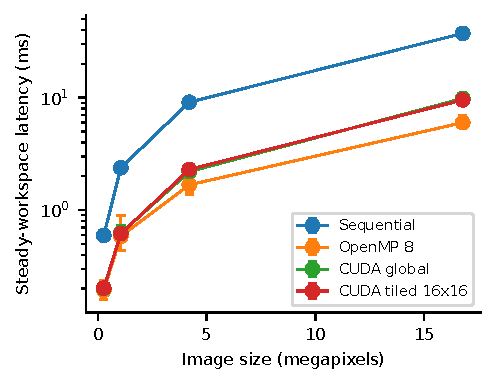
\includegraphics[width=\columnwidth]{figures/latency.pdf}
\caption{Sobel pipeline latency. Error bars show pooled Q1--Q3, not confidence intervals. All staging and transfers are included.}
\label{fig:latency}\end{figure}

At $4096\times4096$, pooled Canny medians are \CannySeq{} ms sequentially and \CannySixteen{} ms with 16 threads. Scaling is not monotonic across the measured thread settings. The global serial queue, allocation behavior, image content and operating-system scheduling are plausible contributors, but this experiment does not isolate their causal effects. Figure~\ref{fig:scaling} uses per-family speedups to avoid equating a ratio of pooled timings with a pooled speedup.
\begin{figure}[t]\centering
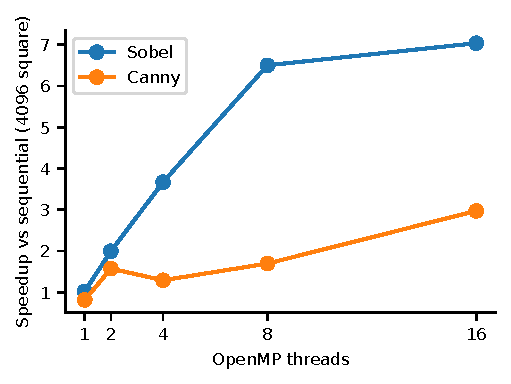
\includegraphics[width=\columnwidth]{figures/scalability.pdf}
\caption{Median of three per-family speedups at $4096\times4096$. The baseline is the same family's sequential implementation.}
\label{fig:scaling}\end{figure}

\subsection{Tiling and data movement}
For baseline CUDA at the largest size, median event intervals are \HtoDLarge{} ms H2D, \KernelLarge{} ms kernel and \DtoHLarge{} ms D2H. The wall median is \CudaLarge{} ms. Differences include host staging, merging and runtime overhead; sums of separate medians need not equal the median of their sum. The tiled $16\times16$ kernel takes \TileKernelLarge{} ms, compared with \KernelLarge{} ms for the global-memory kernel. Every tested tiled shape has a higher pooled kernel median than baseline at every measured resolution (Fig.~\ref{fig:tiling}).

Some tiled pipeline medians are nevertheless slightly lower. Since their kernel work is slower and separately randomized runs have visible spread, these differences do not demonstrate a beneficial tiling optimization. Cache reuse in the baseline and tile-loading/barrier overhead are possible explanations for kernel behavior, but counters were not collected to establish a bottleneck.
\begin{figure}[t]\centering
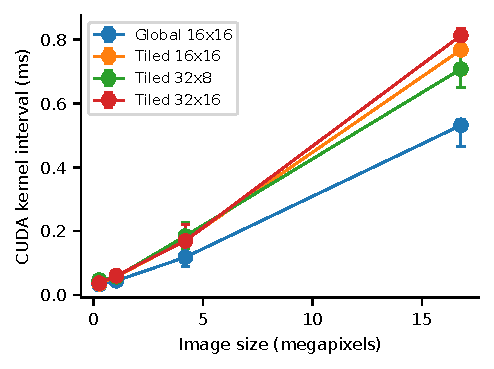
\includegraphics[width=\columnwidth]{figures/tiling.pdf}
\caption{Device event intervals for global and tiled Sobel. Quartile bars summarize all three families. Tiling is a candidate whose measured kernel performance is unfavorable here.}
\label{fig:tiling}\end{figure}

\subsection{Partitions and prediction}
Within the hybrid wrapper, pooled best tested CPU fractions are 1.0, 0.75, 1.0 and 0.5 as width increases. At width 4096, the half-CPU split has a \HybridHalf{} ms median, versus \HybridGpu{} ms at the GPU endpoint and \HybridCpu{} ms at the CPU endpoint. However, independently measured eight-thread OpenMP is \OmpLarge{} ms. The small within-wrapper gain over its CPU endpoint therefore does not establish superiority over a well-performing CPU-only execution (Fig.~\ref{fig:partition}). Endpoint differences across separate processes expose sensitivity to execution context.

The initial throughput estimate does not always select the best tested fraction. Across the recorded family--size combinations, nearest-grid selection has regret from 0 to \RegretMax{}\% relative to the lowest observed candidate median. This is a retrospective diagnostic, subject to selection bias and measurement noise, not out-of-sample policy performance.

\OverlapCount{} hybrid observations have an overlap lower bound greater than 0.01 ms; the largest bound is \OverlapMax{} ms. This supports limited interval overlap in those observations. It does not establish overlap for every configuration or explain latency improvements causally. A synchronized profiler trace would strengthen this validation.

The fitted model yields \ModelError{}\% held-out MAPE on the 15 largest-resolution medians. Figure~\ref{fig:model} shows individual predictions. The held-out set uses the same three synthetic families and hardware, so this result demonstrates size extrapolation within the study only. It does not establish a portable allocation model or justify selecting arbitrary unmeasured fractions.
\begin{figure}[t]\centering
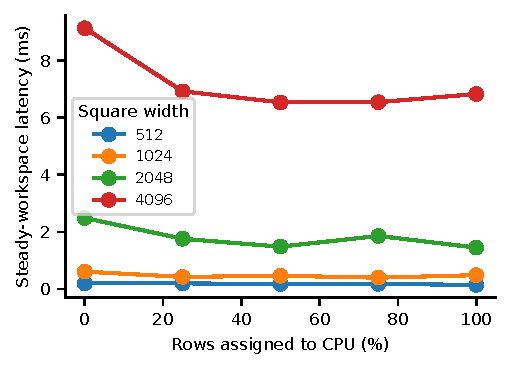
\includegraphics[width=\columnwidth]{figures/partition.pdf}
\caption{Pooled hybrid-wrapper medians across CPU fractions. Endpoint paths and separately timed standalone implementations must be distinguished.}
\label{fig:partition}\end{figure}
\begin{figure}[t]\centering
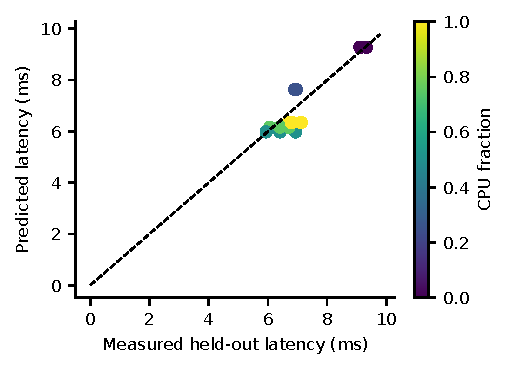
\includegraphics[width=\columnwidth]{figures/prediction.pdf}
\caption{Largest-resolution medians were excluded from fitting. Dashed line denotes exact prediction; color identifies CPU fraction.}
\label{fig:model}\end{figure}

\section{Discussion}
The primary finding is a difference between where arithmetic runs quickly and where an entire host-to-host image operation runs quickly. For a small regular stencil, device computation is only part of the pipeline. Keeping intermediate data resident on the GPU could change this balance, but it would answer a different question and is not measured here.

Adding shared-memory traffic and synchronization can cost more than the reuse it enables. The observed result should inform a future optimization choice, not be hidden by emphasizing a favorable isolated wall-time sample. Similarly, collaborative CPU--GPU execution should be compared against both endpoints under repeated controlled conditions. Merely demonstrating correctness and asynchronous submission is insufficient to claim a practical gain.

The model is useful as a compact description of this dataset, while the rate-estimate regret demonstrates the limits of idealized divisible-work assumptions. The extensive scheduling literature provides stronger general techniques; our study instead makes the timing scope and the limits of a small empirical model inspectable.

\section{Threats to Validity and Limitations}
This is one laptop and one session. The desktop GPU is shared, CPU placement is uncontrolled, and background activity, thermal state and power policy can affect measurements. Fifteen within-process repetitions characterize local variability without establishing cross-day reproducibility. Table~\ref{tab:spread} reports the largest-resolution spread so that small differences are not mistaken for robust improvements.
\begin{table}[t]\centering\footnotesize
\caption{Largest-resolution Sobel latency variability (ms). Q1--Q3 combines image-family and timing variation.}
\label{tab:spread}\begin{tabular}{lrrr}
\hline
Configuration & Median & Q1--Q3 & $n$ \\
\hline
Sequential & 37.318 & 36.489--40.950 & 45 \\
OpenMP 8 & 5.996 & 5.440--6.864 & 45 \\
CUDA global & 9.839 & 9.049--10.443 & 45 \\
CUDA tiled 16x16 & 9.542 & 9.101--9.919 & 45 \\
\hline
\end{tabular}\end{table}

Only synthetic images are measured. Natural-image generalization, different machines, energy, GPU-resident pipelines, cold-start latency and production-library baselines remain untested. CPU SIMD tuning is not explicitly optimized. OpenMP Canny retains a serial queue and includes intermediate allocation costs; CUDA and hybrid Canny are not implemented. Exact comparison validates the specified algorithms, not perceptual edge quality or agreement with every library. Tests cannot prove absence of all memory errors, and Compute Sanitizer was not run.

The model uses a small, structured dataset and configuration medians. MAPE alone does not validate an allocation decision, and no statistically significant or universally optimal partition is claimed. The review verifies source existence and records reading depth, but is not an exhaustive systematic review. Author information and human validation remain required before submission.

\section{Conclusion and Future Work}
Under the specified host-to-host timing contract, OpenMP with eight threads outperforms baseline CUDA Sobel at the largest tested size, despite a short CUDA kernel interval. Shared-memory tiling worsens kernel time in all tested configurations. Hybrid allocation depends on image size and execution context; the evidence does not support a general advantage over CPU-only execution. A small model extrapolates to the held-out largest size with \ModelError{}\% MAPE, within a deliberately narrow scope.

Next steps are independent measurement sessions, controlled power and affinity, natural images with documented licenses, profiler-confirmed overlap, allocation-inclusive latency, and GPU Canny with validated global connectivity. These extensions are required before broader performance or scheduling claims.

\section*{AI Assistance Disclosure}
OpenAI Codex assisted with implementation, experiment orchestration, analysis scripts and manuscript drafting. Measurements were produced by executed programs, not generated timing values. This draft still requires human review of the code, evidence, authorship, and venue-specific disclosure requirements; no submission or acceptance is represented.
\IEEEtriggeratref{17}
\bibliographystyle{IEEEtran}
\bibliography{references}
\end{document}

